\subsection{Вероятностное пространство. Случайные величины. Закон больших чисел в форме Чебышева.}

\centerline{\textbf{Вероятностное пространство}}

\textbf{Пространство элементарных исходов $\Omega$} -- любое непустое множество, содержащее все возможные результаты случайного эксперимента.

Элементы $\omega \in \Omega$ -- \textbf{элементарные исходы} -- исходы случайного эксперимента, из которых в эксперименте происходит ровно один. 

Множество $\mathcal{F}$, элементами которого являются подмножества множества $\Omega$ (не обязательно все) называется \textbf{$\sigma$-алгеброй} (сигма-алгеброй), если выполнены следующие условия:

1. $\Omega \in \mathcal{F}$;

2. если $A \in \mathcal{F}$, то $\neg A \in \mathcal{F}$;

3. $A_1,A_2,\dots~\in \mathcal{F} \implies \bigcup_{i=1}^{\infty} A_i \in \mathcal{F}$ (объединение по \textit{счетному} числу подмножеств)


Минимальная $\sigma$-алгебра, содержащая множество всех интервалов на вещественной прямой, называется \textbf{борелевской $\sigma$-алгеброй} в $\mathbb{R}$ и обозначается $\mathcal{B}(\mathbb{R})$. 

\textbf{Борелевское множество} --- элемент борелевской $\sigma$-алгебры.

\textbf{Вероятность} $P$ --- действительная функция случайного события: $\mathcal{F} \rightarrow \mathbb{R}$, удовлетворяющая следующим условиям:

1. $P(\Omega) = 1$;

2.  $\forall A \in \mathcal{F}\implies P(A) \geqslant 0$;

3. $\forall A_1,A_2,\dots,A_n,\dots \in \mathcal{F}:~A_i \cap A_j = \varnothing (i \neq j) \implies P(\displaystyle\bigcup_{i=1}^{\infty}A_i) = \displaystyle\sum_{i=1}^{\infty}P(A_i)$ (счётная аддитивность).


\textbf{Вероятностное пространство} -- тройка ($\Omega, \mathcal{F}, P$), где $\Omega$ -- множество элементарных исходов, $\mathcal{F}$ -- $\sigma$-алгебра над $\Omega$, вероятность $P$ определена на $\mathcal{F}$.

\textbf{Пример: }
Пусть $\Omega = (\omega_1,\dots,\omega_s)$, $\mathcal{F}$ --- всевозможные подмножества множества $\Omega$.

$P(\omega_1) = \dots = P(\omega_s) = \frac{1}{s} \implies P(A) = \frac{|A|}{|\Omega|}$ --- классическое определение вероятности.

\centerline{\textbf{Случайные величины}}

Пара $(X, \mathcal{U})$, где X – произвольное множество, а $\mathcal{U}$ -- $\sigma$-алгебра над ним -- \textbf{измеримое пространство}. 

Например, $(\Omega, \mathcal{F})$ и $(R, \mathcal{B})$ -- измеримые пространства. 

Элементы  $\sigma$-алгебры $\mathcal{U}$ называются \textbf{измеримыми множествами}.

Пусть даны измеримые пространства $(\Omega, \mathcal{F})$ и $(R, \mathcal{B})$. Функция $\xi : \Omega \rightarrow R$ называется \textbf{случайной величиной}, если прообраз любого борелевского множества $B \in \mathcal{B}$ является событием.

\textbf{Распределением} случайной величины $\xi$ называется функция $P_{\xi}:~\mathcal{B} \rightarrow \mathbb{R}$, определенная $\forall B \in \mathcal{B}$ по правилу $P_{\xi}(B) = P(\xi \in B)$.

\textbf{Функцией распределения} случайной величины $\xi$ называется отображение $F_{\xi}:~\mathbb{R} \rightarrow \mathbb{R}$, определённое по правилу: $F_{\xi}(x) = P(\xi < x)$ или $F_{\xi}(x) = P_{\xi}((-\infty, x))$.

Случайная величина $\xi$ называется \textbf{дискретной случайной величеной}, если существует не более чем счетное множество $B$ такое, что $P_{\xi}(B) = 1$. Распределение, соответствующее дискретной случайной величине, также называется дискретным.

\textit{Дискретная функция распределения} имеет вид:
    \begin{equation*}
        F_\xi(x) = P(\xi < x) = \sum\limits_{x_i < x}{}p_{i} = \sum\limits_{x_i < x}{} P(\xi = x_{i}).
    \end{equation*}


Распределение $\xi$ называется \textbf{абсолютно непрерывным}, если существует
$f(x) \geqslant 0$ такая, что для любого борелевского множества $B$ справедливо
\begin{equation*}
    P_\xi(B) = \int\limits_B f(x) \lambda(dx),
\end{equation*}
где $f(x)$~--- \textit{плотность распределения}, $\lambda$~--- мера Лебега. 
\textit{Абсолютно непрерывная функция распределения} имеет вид:
\begin{equation*}
    F_\xi(x) = P(\xi < x) = \int\limits_{-\infty}^x f(t)dt.
\end{equation*}


\textbf{Пример}: равномерное распределение
$f(x) = \begin{cases}\frac{1}{b - a},& x\in[a,b]\\ 0,& x\notin[a,b] \end{cases}$

% \begin{figure}
    % \centering
    % 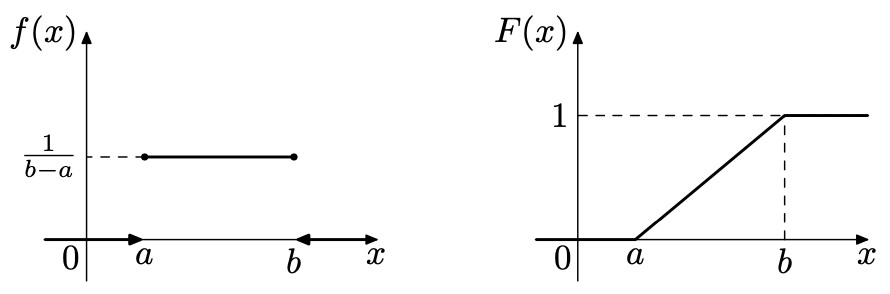
\includegraphics[width=0.01\textwidth]{pics/abs.png}
    % \caption{Пример равномерного распределения}
    % \label{abs}
% \end{figure}
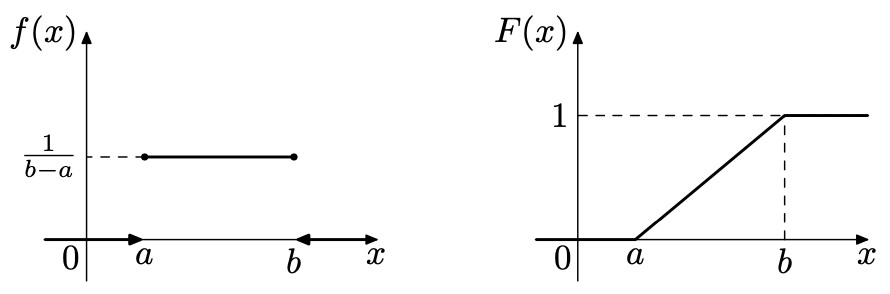
\includegraphics[width=\columnwidth]{pics/abs.png}


\textbf{Математическим ожиданием} случайной величины $\xi$ называется число $E\xi = \int\limits_{\Omega} \xi(\omega) P(d\omega)$ или $\int\limits_{-\infty}^{+\infty} x dF_{\xi}(x)$.
Если интеграл расходится, то говорят, что математического ожидания не существует.

В случае дискретной сл. вел.: $E\xi = \displaystyle\sum_{i} x_i p_i$.

В случае абсолютно непрерывной сл. вел.: $E\xi = \int x f(x) dx$

\textbf{Дисперсией} случайной величины $\xi$ называется число $D\xi = E(\xi - E\xi)^2$, $\sigma = \sqrt{D \xi}$ -- \textbf{среднеквадратическое отклонение}.

% Пусть $\xi$ и $\eta$ -- случайные величины. 
% Дисперсия их суммы в общем случае равна $D(\xi+n)=D \xi+D \eta + 2 \bigl( E (\xi \eta)-E \xi \, E \eta \bigr)$. 
Величина $\operatorname{cov}(\xi, \eta) \equiv E (\xi \eta)-E \xi \, E \eta$ называется \textbf{ковариацией} случайных величин $\xi$ и $\eta$. Если $\xi$ и $\eta$ независимы, то $\operatorname{cov}(\xi, \eta) = 0$. Обратное, вообще говоря, неверно.


\centerline{\textbf{Закон больших чисел в форме Чебышева}}

\textbf{Неравенство Чебышёва}
Если $\exists D\xi$, то $\forall \varepsilon > 0$
\begin{equation*}
    P(|\xi-E \xi| \geqslant \varepsilon) \leqslant \frac{D \xi}{\varepsilon^{2}}.
\end{equation*}


\begin{proof}
    Для $\varepsilon > 0$ неравенство $|\xi - E \xi| \geqslant \varepsilon \iff (\xi - E \xi)^2 \geqslant \varepsilon^2$, поэтому $P(|\xi-E \xi| \geqslant \varepsilon) = 
        P\left((\xi-E \xi)^{2} \geqslant \varepsilon^{2}\right) \leqslant 
        \cfrac{E (\xi-E \xi)^{2}}{\varepsilon^{2}} =
        \cfrac{D \xi}{\varepsilon^{2}}$.
\end{proof}

\textbf{Следствие}:
Если $\varepsilon = 3\sigma$, где $\sigma$ --- стандартное отклонение, то получим
\begin{equation*}
    P\bigl( |\xi-E \xi|> 3 \sigma \bigr) \leqslant 
    \frac{D \xi}{9 \sigma^2} = 
    \frac{D \xi}{9 \, D \xi} =
    \frac{1}{9} \iff 
    P\bigl( |\xi-E \xi| \leqslant 3 \sigma \bigr) \geqslant 
    1-\frac{1}{9} = 
    \frac{8}{9}.
\end{equation*}
Это соотношение называется \textbf{правилом трёх сигм}.

Последовательность случайных величин $\{\xi_n\}_{n = 1}^{+\infty}$ 
\textbf{сходится по вероятности} к случайной величине $\xi$ ($\xi_n \xrightarrow[]{\text{P}} \xi$), если
$$
    \forall \varepsilon>0 \quad P \biggl( \Bigl\{ \omega \colon |\xi_{n}(\omega)-\xi(\omega)|>\varepsilon \Bigr\} \biggr) \xrightarrow[n \to +\infty]{} 0.
$$

\textbf{Закон больших чисел в форме Чебышёва}:
$\forall$ последовательности $\xi_1, \xi_2, \ldots$ попарно независимых и одинаково распределённых случайных величин для которых $E \xi_i^2 < \infty \implies$ 
\begin{equation*}
    \frac{\xi_{1}+\ldots+\xi_{n}}{n} \xrightarrow[n \to + \infty]{\text{P}} E \xi_{1}.
\end{equation*}


\begin{proof}
    $S_n = \xi_1 + \ldots + \xi_n$, Из линейности матожидания получим
    \begin{equation*}
        E \left(\frac{S_{n}}{n}\right)=\frac{E \xi_{1}+\ldots+E \xi_{n}}{n}=\frac{n E \xi_{1}}{n}=E \xi_{1}.
    \end{equation*}
    
    Пусть $\varepsilon > 0$. Воспользуемся неравенством Чебышёва:
    \begin{multline*}
        P\left(\left|\frac{S_{n}}{n}-E \left(\frac{S_{n}}{n}\right)\right| \geqslant \varepsilon\right) \leqslant \frac{D\left(\frac{S_{n}}{n}\right)}{\varepsilon^{2}}
        = \frac{D S_{n}}{n^{2} \varepsilon^{2}}
        = \frac{D \xi_{1}+\ldots+D \xi_{n}}{n^{2} \varepsilon^{2}}= \\
        = \frac{n D \xi_{1}}{n^{2} \varepsilon^{2}}
        = \frac{D \xi_{1}}{n \varepsilon^{2}} \xrightarrow[n \to +\infty]{} 0,
    \end{multline*}
    т.к. $D\xi_1 < \infty$. Дисперсия суммы превратилась в сумму дисперсий в силу попарной независимости слагаемых, из-за которой все ковариации $\operatorname{cov}(\xi_i, \xi_j)$ по свойству ковариации обратились в нуль при $i \neq j$.
\end{proof}


\textbf{Центральная предельная теорема}:
    Пусть $\xi_{1}, \xi_{2}, \ldots$~--- последовательность независимых одинаково распределенных невырожденных случайных величин с $E \xi_{1}^{2}<\infty$ и $S_{n}=\xi_{1}+\ldots+\xi_{n}$. 
    Тогда
    \begin{equation*}
        P\left(\frac{S_{n}-E S_{n}}{\sqrt{D S_{n}}} \leqslant x\right)
        \xrightarrow[n \to +\infty]{}
        \Phi(x) = \frac{1}{\sqrt{2 \pi}} \int\limits_{-\infty}^{x} e^{-\frac{u^{2}}{2}} du~~ \forall x \in R
    \end{equation*}

\begin{proof}
Пусть $E \xi_{1}=m,\, D \xi_{1}=\sigma^{2}$. 
Введём $X = \xi_1 - m$ и $D \phi_X(t)=E e^{i tX}$ и 
$
    D \phi_{n}(t)=E e^{i t \frac{S_{n}-E S_{n}}{\sqrt{D S_{n}}}} = 
    \left[D \phi_X\left(\frac{t}{\sigma \sqrt{n}}\right)\right]^{n}
$

В силу разложения характеристической функции (при $\exists$ соответствующих моментов)
$
    D \phi_{X}(t)=1+i t E X+\ldots+\frac{(i t)^{n}}{n !} E X^{n}+R_{n}(t)
$

Т.к. $E X = E \left[ \xi_1 - m\right] = 0$, при $n=2$: 
$
    D \phi(t)=1-\frac{\sigma^{2} t^{2}}{2}+\overline{o}\left(t^{2}\right), \quad t \to 0
$.

$\forall t \in R$ при $n \to +\infty \implies $
$
    D \phi_{n}(t)=\left[1-\frac{\sigma^{2} t^{2}}{2 \sigma^{2} n}+\overline{o}\left(\frac{1}{n}\right)\right]^n \to e^{-\frac{t^{2}}{2}}
$

Функция $e^{-\frac{t^{2}}{2}}$ -- характеристическая функциия $N_{0,1}$. 
В силу теоремы о непрерывном соответствии между функциями распределения и характеристическими функциями Ц.П. теорема доказана.
\end{proof}

% -------- source --------
\bigbreak
[\cite[page 1-53]{stat_book}]